\setcounter{figure}{0}
\setcounter{table}{0}
\setcounter{equation}{0}

\irsection{Combustion and Ignition at the Propellant Surface}{Ibiricu}

Before presenting the theory behind the \Rocburn\ implementation, this section discusses the ideas of propellant combustion and ignition more broadly. The thermal transient theory inside \Rocburn\ is abstract, so presentation of this broader picture will help to concretize the physical phenomena taking place in the different regions, each modeled in its own way. The following figure and associated description are taken directly from [\cite{Ibiricu:1975}].

\begin{figure}[ht]
\centering
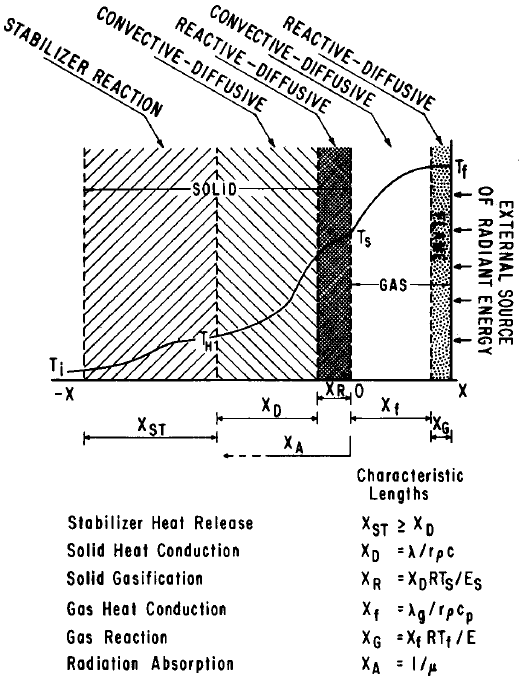
\includegraphics[width=0.5\textwidth]{../Figures/IbiricuCombustionModel.png}
\caption{Schematic illustration of combustion model from [\cite{Ibiricu:1975}]. Variable descriptions: solid thermal conductivity, $\lambda$; burn rate, $r$; density, $\rho$; solid heat capacity per unit mass, $c$; universal gas constant, $R$; temperature of solid surface, $T_s$; activation energy for solid phase reaction, $E_s$; gas thermal conductivity, $\lambda_g$; gas specific heat at constant pressure, $c_p$; flame temperature, $T_f$; activation energy for gas phase reaction, $E$; and absorption coefficient for solid, $\mu$.}
\label{fig:ibiricu}
\end{figure}

\begin{quote}
The combustion model is illustrated schematically in \irref{Figure}{fig:ibiricu}. The solid phase occupies the region $x < 0$ and the gas phase the region $x > 0$. Externally provided radiation is incident on the propellant from the gas. The temperature profile has been drawn for the unperturbed state of zero radiant flux. Allowance is made for gaseous and solid reactions, each being presumed to have activation energies
sufficiently high for reactive--diffusive and convective--diffusive zones to be identifiable [\cite{Williams:1973}]. In addition, a stabilizer reaction zone is included for propellants containing stabilizers that react exothermically at low temperatures [\cite{Huggett:1960,Kovalskii:1967}]. Regression rates are assumed to be controlled by the gaseous or solid reaction, or by a combination thereof, but not by the stabilizer reaction, whose effect is treated purely energetically.

Although it may not be apparent, the model encompasses conventional views of double-base propellant combustion [\cite{Huggett:1960}]. The convective--diffusive zone in the gas may represent the ``dark zone,'' and the reactive--diffusive zone in the solid is a combination of the subsurface and ``fizz'' reaction zones of the classical description. Placement of the surface on the hot side of this last zone, and calling it the ``solid reaction zone'' are merely conventions ... Experimental demarkation of a boundary between subsurface and fizz zones is inconclusive, and two-phase flow analyses needed in attempting to resolve the issue are very difficult. If the demarkation can be achieved, then a boundary temperature can be identified which conventionally has been called the ``surface temperature'' and which lies below the $T_s$ of \irref{Figure}{fig:ibiricu} when the reactive--diffusive zone of the solid encompasses the fizz zone. Since rates of fizz-zone reactions may be expected to depend on pressure, there should be no hesitance to assign pressure dependence to rates in the present ``solid reaction zone.'' The model is capable of retaining or excluding the break in the temperature curve shown at $x=0$.  [\cite{Ibiricu:1975}]
\end{quote}